\begin{frame}\frametitle{Performance of the MODIS semi-analytical ocean color algorithm for chlorophyll-a} 
\scriptsize
\begin{description}
    \item[Authors] K.L. Carder, F.R. Chen, J.P. Cannizzaro, J.W. Campbell, B.G. Mitchell
    \item[Objectives] Test effectiveness of MODIS semi-analytical algorithm (Chlor\_a\_3) against previous chlorophyll--a measurements from CZCS and SeaWiFS - particularly for high latitudes and regions with strong overturn, where chlorophyll-a (Chla) concentrations have been severely underestimated.
    
    \item[Methods] 
        \begin{itemize}
            \item Separation of the chlorophyll-specific phytoplankton absorption coefficient, $a^{\ast}_{ph}(\lambda)$ from gelbstoff/detritus for more accurate measures of chlorophyll-a.
            \item Previous algorithms for measuring chlorophyll concentration relied on the strong positive dependencies between the phytoplankton absorption coefficient at 440 nm and 675 nm, $a_{ph}(440, 675)$, and Chla. The SA algorithm is exceptional because it accommodates high degrees of variability of $a^{\ast}_{ph}(\lambda)$ in high-latitude/strong upwelling zones.
        \end{itemize}
\end{description}
\end{frame}

\begin{frame}\frametitle{Performance of the MODIS semi-analytical ocean color algorithm for chlorophyll-a} 
\scriptsize
\begin{description}
    \item[Findings]
        \begin{itemize}
            \item Chla can be accurately measured by empirical algorithms for $a_{ph}(675)$ $>$ 0.03 m-1, or 1.5 -2.0 mg/m3, but the semi-analytical algorithm is necessary for $a_{ph}(675)$ $<$ 0.03 m-1.
            \item near 1:1 relationship between SA modeled Chla and in situ Chla measurements, with significantly worse performance from modeled Chla using the empirical Chlor\_a\_2 algorithm (0.5:1, and 0.7:1 underestimations for two different study areas). 
            \item Chlor\_a\_2 and Chlor\_a\_3 both tend to agree with their estimations of Chla in equatorial waters, with the exception of zones of strong upwelling equatorial waters in the Eastern Pacific.
            \item The SA algorithm showed lower concentrations in chlorophyll-a than Chlor\_a\_2 in parts of the northern hemisphere because it was more effective at distinguishing between gelbstoff-rich runoff from northern rivers and ocean chlorophyll.
            \item One the most noticeable differences in Chla values is in high-latitude waters in the southern hemisphere during austral spring, where chlorophyll concentration in phytoplankton blooms was misrepresented by Chlor\_a\_2 because of chlorophyll packaging. 
        \end{itemize}
\end{description}

  \note[item]{Include notes and talking points here.}
  \note[item]{There can be more than one note.}
\end{frame}

\begin{frame}\frametitle{Performance of the MODIS semi-analytical ocean color algorithm for chlorophyll-a} 
    \begin{center}
        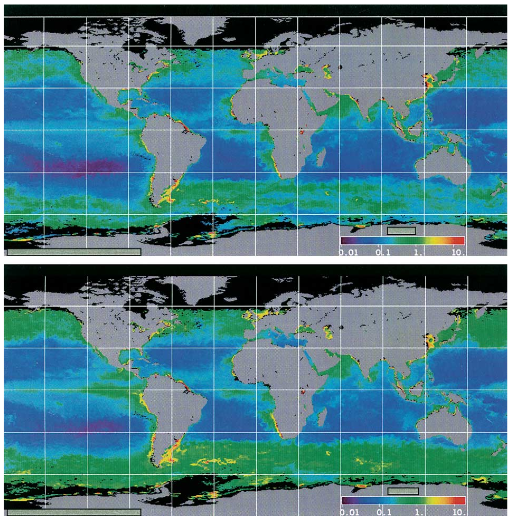
\includegraphics[width=\textwidth,height=0.7\textheight,keepaspectratio]{carder}

\tiny Global maps (December 2000) of chlorophyll--$a$ concentration ($mg$ $m^{-3}$) composited in 39 km bins retrieved using empirical (Chlor\_a\_2, top) and semi-analytical (Chlor\_a\_3, bottom algorithms from MODIS Terra radiometry.
    \end{center}
  \note[item]{Pretty picture}

\end{frame}
